\documentclass{beamer}
%\usepackage{xspace}
\usepackage{amsmath,amssymb}
\usepackage{graphicx}
%\usepackage{svg}
%\usepackage{pgfpages}
%\pgfpagesuselayout{4 on 1}[a4paper,border shrink=5mm,landscape]
%\usepackage{psfrag}
%\usepackage[usenames,dvipsnames]{xcolor}
\usepackage{braket}
\usepackage{qcircuit}
\usepackage{tikz}
\usetikzlibrary{circuits.logic.US}
\usetikzlibrary{graphs}
\usetikzlibrary{datavisualization}
\usetikzlibrary{datavisualization.formats.functions}
\usepackage{pgfplotstable}
\usepgfplotslibrary{patchplots}

\setbeamercovered{transparent}

\usetheme{Pittsburgh}
%\usetheme{default}

\setbeamertemplate{sidebar right}{}
\setbeamertemplate{footline}[frame number]
%\usefonttheme{professionalfonts}

%\usepackage{sansmathaccent}
%\usepackage{bm}

%\usepackage{unicode-math}
%%\setmainfont[SlantedFont={Latin Modern Roman Slanted},SlantedFeatures={Color=000000},
%%  SmallCapsFont={TeX Gyre Termes},SmallCapsFeatures={Letters=SmallCaps}]{XITS}
%\setmathfont[math-style=ISO,sans-style=upright]{XITS Math}
%\setmathfont[range={\mathcal,\mathbfcal}]{Latin Modern Math}

\usepackage{sfmath}

%\mathversion{sans}

\newcommand{\Tr}{\mathsf{Tr}}

\definecolor{redorange}{rgb}{1.0, .25, .25}
\definecolor{citation}{rgb}{.1, 0.8, .35}
\newcommand\emm[1]{\textcolor{redorange}{{#1}}}
\newcommand\numc[1]{\textcolor{citation}{{\bf #1}}}

%\newcommand\bm[1]{{\mbox{\boldmath $#1$}}}
\newcommand\bm[1]{{\mathbf{#1}}}
%\newcommand\bm[1]{{\bf #1}}
%\newcommand\bm[1]{\ensuremath{\boldsymbol{#1}}}
%\newcommand\bm[1]{{\textbf{\it #1}}}

\title{No-signaling polytope and multiplayer XOR games}
\author{Ryuhei Mori}
%\institute{$\vcenter{\hbox{\includegraphics[width=30pt]{ELC_logo}}}$ Postdoctoral Fellow of ELC\\ $\vcenter{\hbox{\includegraphics[width=20pt]{titech_logo}}}$ Tokyo Institute of Technology}
\institute{Tokyo Institute of Technology}
%\date{21, Feb, 2019}



\begin{document}
\begin{frame}[plain]
\maketitle
\end{frame}



\begin{frame}{Boolean circuit}
\begin{itemize}
\setlength{\itemsep}{2em}
\item Boolean function $f\colon \{0,1\}^n\to\{0,1\}$.
\item \emm{Boolean circuit} is a model of computation which consists of \emm{gates}.
\item AND gate:
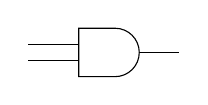
\begin{tikzpicture}[circuit logic US, baseline]
\node[and gate] (A) {};
\foreach \a in {1, 2}
  \draw (A.input \a -| -1,0) -- (A.input \a);
\draw (A.output) -- ([xshift=0.5cm]A.output);
\end{tikzpicture}
\item OR gate:
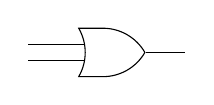
\begin{tikzpicture}[circuit logic US, baseline]
\node[or gate] (A) {};
\foreach \a in {1, 2}
  \draw (A.input \a -| -1,0) -- (A.input \a);
\draw (A.output) -- ([xshift=0.5cm]A.output);
\end{tikzpicture}
\item NOT gate:
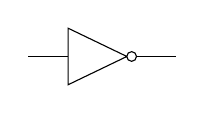
\begin{tikzpicture}[circuit logic US, baseline]
\node[not gate] (A) {};
\draw (A.input) -- ([xshift=-0.5cm]A.input);
\draw (A.output) -- ([xshift=0.5cm]A.output);
\end{tikzpicture}
\end{itemize}
\end{frame}

\begin{frame}{Universality of $\{\mathsf{AND}, \mathsf{OR},\mathsf{NOT}\}$}
\begin{theorem}
For any Boolean function $f\colon \{0,1\}^n\to\{0,1\}$, there is a Boolean circuit with AND, OR and NOT gates computing $f$.
\end{theorem}
\begin{proof}
The proof is induction on $n$. Theorem is trivial for $n=1$.
Assume that Theorem holds for Boolean functions $n \le k-1$.
\begin{align*}
f(x_1,\dotsc,x_n) = (x_n \wedge f(x_1,\dotsc,x_{n-1}, 1)) \vee (\overline{x_n} \wedge f(x_1,\dotsc,x_{n-1}, 0))
\end{align*}
\end{proof}
\end{frame}

\begin{frame}{Size of Boolean circuit}
Size of Boolean circuit $:=$ \# of gates in the Boolean circuit.

Let $C(f)$ be a smallest size of Boolean circuit computing $f\colon\{0,1\}^n\to\{0,1\}$.

Let $s(n) := \max_{f\colon\{0,1\}^n\to\{0,1\}} C(f)$.

\begin{align*}
f(x_1,\dotsc,x_n) = (x_n \wedge f(x_1,\dotsc,x_{n-1}, 1)) \vee (\overline{x_n} \wedge f(x_1,\dotsc,x_{n-1}, 0))
\end{align*}
\begin{align*}
s(n) &\le c + 2 s(n-1)\\
\frac{s(n)}{2^n} &\le \frac{c}{2^n} + \frac{s(n-1)}{2^{n-1}}\\
&\le c \left(\frac1{2^n} + \frac1{2^{n-1}} + \dotsb \frac12\right) + s(0) \le c + s(0)
\end{align*}
\begin{center}
\begin{equation*}
s(n) = O(2^n)
\end{equation*}
\end{center}
\end{frame}

\begin{frame}{Lower bound of size of Boolean circuit}
The number of Boolean functions with $n$ variables is $2^{2^n}$.

\vspace{1em}
The number of Boolean circuits of size $s$ is at most
\begin{equation*}
\left(8\binom{n+s}{2}\right)^s
\le (8(n+s)^2)^{s}.
\end{equation*}

This means
\begin{align*}
& (8(n+s(n))^2)^{s(n)}\ge 2^{2^n} \\
\iff& {s(n)}\log(8(n+s(n))^2)\ge 2^n\\
\Longrightarrow& s(n)\ge \frac{2^n}{n}
\end{align*}
\end{frame}

\begin{frame}{Quantum circuit}
\begin{itemize}
\setlength{\itemsep}{1.5em}
\item Unitary operator $U\in L(\mathbb{C}^{2^n})$.
\item \emm{Quantum circuit} is a model of computation which consists of \emm{quantum gates}.
\item Single qubit gate: $X$ gate, $Y$ gate, $Z$ gate, $H$ gate, $S:=\begin{bmatrix}1&0\\0&i\end{bmatrix}$ gate
%\[
\Qcircuit @C=2em @R=.7em {
& \gate{X} & \qw
}
%\]
\item Two qubit gate: CNOT gate
\Qcircuit @C=2em @R=1em {
& \ctrl{1} & \qw\\
& \targ & \qw
}
\item Three qubit gate: Toffoli gate
\mbox{
\Qcircuit @C=2em @R=1em {
& \ctrl{1} & \qw\\
& \ctrl{1} & \qw\\
& \targ & \qw
}
}
\end{itemize}
\end{frame}

\begin{frame}{``Classical computation'' by a quantum circuit}
\begin{lemma}
For any function $F\colon \{0,1\}^n\to\{0,1\}^m$,
%With sufficiently large number of working qubits (ancilla),
there is a quantum circuit on $n+m+w$ qubits which consists of \emm{$X$} and \emm{Toffoli} gates for $U$ satisfying
\begin{equation*}
U\ket{x}\ket{y}\ket{0}^{\otimes w} = \ket{x}\ket{y\oplus f(x)}\ket{0}^{\otimes w}
\end{equation*}
for all $x\in\{0,1\}^n$, $y\in\{0,1\}^m$.
The number $w$ of ancillary qubits and the number $g$ of quantum gates are at most $C(f)$.
\end{lemma}
\begin{proof}[A sketch of a proof]
Induction on the number of gates.
\end{proof}
\end{frame}

\begin{frame}{Universality of a quantum circuit}
\begin{theorem}[Universality of finite gate set]
For any unitary matrix $U\in L(\mathbb{C}^{2^n})$ and $\emm{\epsilon} >0$,
there is a quantum circuit with \emm{$X,\,Y,\,Z,\,H,\,S,\,\mathsf{CNOT},\,\mathsf{Toffoli}$} gates computing $\widetilde{U}$
satisfying $\|U-\widetilde{U}\|<\emm{\epsilon}$.
\end{theorem}
\begin{proof}
In the next class.
\end{proof}
\end{frame}

\begin{frame}{Oracle model}

\begin{itemize}
\setlength{\itemsep}{2em}
\item Input is given by an oracle.
\item Classical oracle: oracle gate $i\mapsto x_i$.
\item Quantum oracle: quantum oracle gate $O\ket{i}\ket{y} = \ket{i}\ket{y\oplus x_i}$.
\item Query complexity: the number of oracle calls.
\item Circuit size: the number of total quantum gates.
\end{itemize}
\end{frame}

\begin{frame}{Deutsch--Josza problem}
\begin{itemize}
\setlength{\itemsep}{2em}
\item There is a hidden Boolean function $f\colon\{0,1\}^n\to\{0,1\}$ that is a constant or balanced.
\item Quantum oracle $U\ket{x}\ket{y} = \ket{x}\ket{y\oplus f(x)}$.
\item Goal is to determine whether $f$ is constant or balanced.
\item Classical deterministic algorithm needs $2^{n-1}+1$ oracle calls.
\item Deutsch--Josza algorithm solves this problems by \emm{single} oracle call.
\end{itemize}
\end{frame}

\begin{frame}{Deutsch--Josza problem}
\[
\Qcircuit @C=2em @R=1em {
\lstick{\ket{0}} & \gate{H} & \multigate{3}{U} & \gate{H} & \meter\\
\lstick{\ket{0}} & \gate{H} & \ghost{U} & \gate{H} & \meter\\
\lstick{\ket{0}} & \gate{H} & \ghost{U} & \gate{H} & \meter\\
\lstick{\ket{1}} & \gate{H} & \ghost{U} & \gate{H} & \meter\\
}
\]
\begin{align*}
&\ket{0}^{\otimes n}\ket{1}
\stackrel{H^{\otimes (n+1)}}{\longmapsto} \ket{+}^{\otimes n}\ket{-}
= \frac1{2^{n/2}}\sum_{x\in\{0,1\}^n}\ket{x}\ket{-}\\
&\stackrel{U}{\longmapsto} \frac1{2^{n/2}}\sum_{x\in\{0,1\}^n}(-1)^{f(x)}\ket{x}\ket{-}\\
&\stackrel{H^{\otimes (n+1)}}{\longmapsto} \frac1{2^{n}}\sum_{x\in\{0,1\}^n}\sum_{y\in\{0,1\}^n}(-1)^{f(x)}(-1)^{\langle x, y\rangle}\ket{y}\ket{1}\\
\end{align*}
\end{frame}

\begin{frame}{Assignments}
\begin{enumerate}
\setlength{\itemsep}{2em}
\item Show that the PR-box satisfies the no-signaling condition.
\item Show an optimal strategy for the generalized Mermin--GHZ game, defined by
\small
\begin{align*}
p(x_1,\dotsc,x_n) &:= \frac{\mathbb{I}\left\{\sum_{j=1}^n x_j\text{ is divisible by } 2^\ell\right\}}{\left|\left\{z\in\{0,1\}^n\mid \sum_{j=1}^n z_j \equiv 0 \mod 2^\ell\right\}\right|},\\
f(x_1,\dotsc,x_n) &:= \frac{\sum_{j=1}^n x_j}{2^\ell}\mod 2.
\end{align*}
\end{enumerate}
\end{frame}

\end{document}
